\chapter{Analyse des aktuellen Standes der \acl{CE}}
\label{sec:analyse}

\section{\acl{CE}}
\ac{CE} ist sowohl eine Abteilung als auch eine Softwarekomponente der SAP
eigenen HANA-Datenbank \todo{Quelle? Buch SAP HANA die Einführung}. Der genaue Funktionsumfang von HANA ist in dieser
Arbeit nicht weiter relevant.
Eine Möglichkeit um Daten mit der HANA-Datenbank zu analysieren, sind jedoch
sogenannte Kalkulationssichten. Da nur diese Kalkulationssichten in der Arbeit
weiter betrachtet werden, werden sie im Folgenden auch als Datenbankabfragen
bezeichnet. \autocite[Vgl.][]{SapHanaCreateCalcViews} Diese Kalkulationssichten
werden von der \ac{CE} bearbeitet. Das Vorgehen wird in
\autoref{sec:modells_db_queries} genauer beschreiben.


\section{Modelle und Datenbankabfragen}
\label{sec:modells_db_queries}


In der \ac{CE} werden diese Datenbankabfragen durch Modelle dargestellt. Für
jede Abfrage wird zuerst das dazugehörige Modell instanziiert. Anschließend
wird dieses Modell optimiert, um die Ausführungsdauer der Abfrage zu
minimieren. Diese optimierte Abfrage, wird dann auf der Datenbank ausgeführt.
Für die Ausführung ist dabei jedoch nicht zwingend die \ac{CE} zuständig
\autocite[vgl.][]{SapHanaExecutionEngines}.
Allgemein kann man ein Modell als azyklischen gerichteten Graphen nach
\autoref{def:gerichteter_graph} und \autoref{def:zyklen} beschreiben. Des
Weiteren ist zu beachten, dass dieser Graph nur eine Quelle nach
\autoref{def:quelle_senke} hat, welche auch als Abfrageknoten bezeichnet wird.
Diese Definitionen reichen jedoch nicht aus, da zwischen verschiedenen Arten
von Knoten unterschieden wird, welche jeweils verschiedene Informationen
beinhalten.  Allgemein werden die Knoten in der \ac{CE} in zwei Gruppen
unterschieden, Datenquellen und Sichtknoten. Es gibt verschiedene Datenquellen,
zur Vereinfachung werden in dieser jedoch Arbeit nur
\foreignlanguage{english}{Table}-Knoten betrachtet. Deshalb werden Datenquellen
im Folgenden auch Tabellenknoten genannt.
%Ein \foreignlanguage{english}{Table}-Knoten spiegelt eine Tabelle einer Datenbank wider.
Die andere Gruppe sind die Sichtknoten. Zu diesen gehören \zB
\foreignlanguage{english}{Projection}, \foreignlanguage{english}{Aggregation},
\foreignlanguage{english}{Join} und \foreignlanguage{english}{Union}. Auch hier
gibt es zwar noch Weitere, diese Arbeit beschränkt sich jedoch auf diese.
Diese Modelle können zwar wie in \autoref{def:gerichteter_graph}
beschreiben als eine Menge von Knoten und Kanten dargestellt werden, gespeichert wird
jedoch eine Liste an Knoten, von welchen jedem seine Kind- und Elternknoten
zugeordnet sind. Die Kindknoten werden dabei als Eingangsknoten und die
Elternknoten als Ausgangsknoten bezeichnet. Jeder Knoten kann beliebig viele
Ausgangsknoten haben, wobei es wie bereits beschreiben nur einen Knoten mit $0$
Ausgangsknoten gibt. Die Anzahl der Eingangsknoten unterscheidet sich dabei je
nach Knotentyp.
\foreignlanguage{english}{Projection}- und
\foreignlanguage{english}{Aggregation}-Knoten haben genau einen,
\foreignlanguage{english}{Join}-Knoten genau zwei,
\foreignlanguage{english}{Union}-Knoten zwei oder mehr und
\foreignlanguage{english}{Table}-Knoten haben keinen Eingangsknoten.
Bei den Eingangsknoten kann es sich um Tabellenknoten
sowie auch Sichtknoten handeln. \autocite[Vgl.][]{SapHanaSupportedViewNodes}

\autoref{fig:bsp_modell} zeigt ein einfaches Beispielmodell, welches zur
Veranschaulichung dient. Das Modell besteht aus fünf Knoten, dem Abfrageknoten,
zwei Sichtknoten und zwei Tabellenknoten. In dem Knoten steht der Name des
Knotens und neben ihm steht der Knotentyp. Bis auf den Abfrageknoten haben in
diesem Beispiel alle Knoten eine Zahl als Namen. Der Abfrageknoten sowie alle
Tabellenknoten sind zusätzlich farblich markiert. Knoten 1 ist ein
\foreignlanguage{english}{Join}-Knoten. Er hat zwei Eingangsknoten, den
\foreignlanguage{english}{Table}-Knoten 2 und den
\foreignlanguage{english}{Projection}-Knoten 3. Der einzige Ausgangsknoten ist
in diesem Fall der Abfrageknoten, dieser ist hier vom Typ
\foreignlanguage{english}{Aggregation}. Der Abfrageknoten kann jedoch
alternativ auch vom Typ \foreignlanguage{english}{Projection} sein.

\begin{figure}
    \begin{center}
        \begin{tikzpicture}[
    node distance = 1cm,
    request/.style = {rectangle, draw, blue, minimum width=2cm, minimum height=0.8cm},
    op_node/.style = {circle, draw, minimum size=1cm},
    table_node/.style = {circle, draw, magenta, minimum size=1cm},
    arrow/.style = {->, >=stealth}
]

% Nodes
\node[request] (0) at (0,3) {Abfrage};
\node[right=0.2cm of 0] {Aggregation};

\node[op_node] (1) at (0,1) {1};
\node[below=0.2cm of 1] {Join};

\node[table_node] (2) at (-2,-1) {2};
\node[below=0.2cm of 2] {Table};

\node[op_node] (3) at (2,-1) {3};
\node[right=0.2cm of 3] {Projection};

\node[table_node] (4) at (2,-3) {4};
\node[below=0.2cm of 4] {Table};

% Arrows
\draw[arrow] (0) -- (1);
\draw[arrow] (1) to[out=210,in=90] (2);
\draw[arrow] (1) to[out=-30,in=90] (3);
\draw[arrow] (3) -- (4);

\end{tikzpicture}

    \end{center}
    \caption{Darstellung eines Beispielmodells}\label{fig:bsp_modell}
\end{figure}

Zusätzlich zu den Eingangs- und Ausgangsknoten werden in jedem Knoten
noch weitere Informationen gespeichert. Jeder Knoten beinhaltet
eine Liste an Sichtattributen, diese legt fest, welche Sichtattribute dieser
Knoten an seine Ausgangsknoten weitergibt. Bei einem Tabellenknoten sind die
Sichtattribute gleichbedeutend mit den Spalten der Tabelle. Die Sichtattribute
des Abfrageknotens sind die Attribute, welche im Ergebnis der Abfrage enthalten
sind. Damit Sichtattribute umbenannt werden können, wird jedem Eingangsknoten
eine Liste an Mappings zugeordnet. Hat der Knoten $N$ einen Eingangsknoten $E$
mit einem Mapping, dann bildet dieses ein Sichtattribut von $E$ auf ein
Sichtattribut von $N$ ab.

Die verschiedenen Sichtknotentypen sind für verschiedene Operationen zuständig.
Manche dieser Knoten haben noch zusätzliche Attribute, um die genaue Art und
Weise der Operation festzulegen.
Ein \foreignlanguage{english}{Join}-Knoten kann genutzt werden, um die
Ergebnisse der beiden Eingangsknoten zu verbinden. 

% section Modelle und Datenbankabfragen (end)
In der \ac{CE} werden bereits verschiedene Wege genutzt, um die Performance und
das Verhalten der HANA-Datenbank zu analysieren. 
\section{Google Benchmark}
\label{sec:google_benchmark}

Google Benchmark ist ein Open Source Benchmarking Tool von Google,
welches es einem ermöglicht einzelne Funktionen in C++ zu benchmarken. 
Dazu kann man ähnlich zu den meisten Test-Frameworks drei verschiedene
Codeabschnitte definieren.

Der Hauptabschnitt definiert was genau im Benchmark untersucht werden
soll. Diese legt die für die Messung relevante Logik fest.
Der \foreignlanguage{english}{Setup}-Abschnitt wird einmal vor jeder Ausführung des Benchmarks
aufgerufen. In dieser werden die Voraussetzungen für die Ausführung des Hauptabschnitts
geschaffen. Man kann ihn \zB nutzen, um Testdaten für den Benchmark
zu generieren oder zu laden, da er nicht bei den Messungen beachtet wird.
Der \foreignlanguage{english}{Teardown}-Abschnitt wird nach jeder Ausführung des Benchmarks aufgerufen.
Dieser beeinflusst, wie der Setup Abschnitt, die Messung nicht.

Des Weiteren bietet Google Benchmark die Option, einen Benchmark mehrmals mit
unterschiedlichen Parametern durchzuführen. Um beispielsweise die Auswirkung
der Größe des Testdatensatzes auf das Ergebnis zu beobachten.

\autoref{fig:google_benchmark_ausgabe} zeigt eine Beispielhafte Google
Benchmark Ausgabe. Benchmark ist dabei der Name des Benchmarks sowie die werte
der Parameter, welche durch einen Schrägstrich getrennt sind.
\foreignlanguage{english}{Time} und CPU sind beide die durchschnittliche Dauer einer
Ausführung des Hauptabschnitts über alle Iterationen hinweg. Der Unterschied
besteht darin, welche Zeit genau gemessen wird. \foreignlanguage{english}{Time}
ist die tatsächlich benötigte Zeit ist, wobei Wartezeiten des Prozessors
inkludiert sind. CPU ist im hingegen nur die Zeit, welche der Prozessor
wirklich genutzt hat, um den Benchmark-Prozess zu bearbeiten, hierbei sind
Wartezeiten also exkludiert. Dies betrifft sowohl die Wartezeiten, welche durch
das Eingreifen des \foreignlanguage{english}{Scheduler} auftreten
\autocite[vgl.][184]{RoundRobin}, als auch Wartezeiten, welche durch \zB
Speicherzugriffe oder Ein- und Ausgabeoperationen verursacht werden.
\foreignlanguage{english}{Iterations}
ist die Anzahl der durchgeführten Wiederholungen des Hauptabschnitts. Legt man
bei der Definition des Benchmarks keine Anzahl fest, wird die Anzahl der
Wiederholungen anhand der durchschnittlichen Dauer einer Iteration und der
Varianz der Dauer über alle Iterationen hinweg festgelegt.
\autocite[Vgl.][]{GoogleBenchmark}

\begin{figure}[h]
    \begin{center}
        \begin{BVerbatim}

-------------------------------------------------------
Benchmark             Time       CPU        Iterations 
-------------------------------------------------------
BM_Optimizer/8/0      213 us      212 us    3276
BM_Optimizer/16/0     271 us      271 us    2621
BM_Optimizer/32/0     389 us      389 us    1790
BM_Optimizer/64/0     739 us      738 us    1064
BM_Optimizer/128/0    1037 us    1037 us     687
BM_Optimizer/256/0    2372 us    2371 us     319
        \end{BVerbatim}
    \end{center}
    \caption{Beispielausgabe eines Google Benchmarks}\label{fig:google_benchmark_ausgabe} 
\end{figure}
Google Benchmark wird in der \ac{CE} meistens genutzt, um das Verhalten der
Laufzeit bestimmter Funktionen in künstlich generierten Testfällen zu
vergleichen. Hierbei wird keine HANA-Instanz benötigt, da
keine Operationen auf einer Datenbank ausgeführt werden, sondern nur einzelne
Funktionen aufgerufen werden. Es werden folglich
auch keine Testdatensätze für die Datenbank benötigt, sondern nur Daten, auf
welchen man die zu analysierende Funktion aufrufen kann.

Im Vergleich zu anderen Methoden der Performance Messung, die Operationen auf
einer HANA-Instanz ausführen, ist ein Google Benchmark relativ einfach.
Dies liegt daran, dass sie weniger Voraussetzungen erfordern und sich lediglich
auf einen kleinen Teil der Logik konzentrieren.
% section Google Benchmark (end)


\section{HANA-Profiler}
\label{sec:hana_profiler}

Eine weitere Methode die Performance und das Verhalten von Software zu
analysieren ist, das bereits in \autoref{sec:performance_analyse}
beschriebene, Profiling.

In der \ac{CE} wird hauptsächlich der \enquote{BOOSS-Profiler}, ein in HANA
integrierter Profiler, verwendet. Auf diesen kann entweder manuell oder im Code
zugegriffen werden. Dabei sind die wichtigsten Befehle \verb+profiler clear+
um die aktuellen Profilinginformationen zurückzusetzen, \verb+profiler start+
um den Profiler zu starten, \verb+profiler stop+ um den Profiler zu
stoppen und \verb+profiler print+ um die gesammelten Profilinginformationen
auszugeben.

Der Profiler kann in diesem Kontext auf zwei verschiedene Arten genutzt werden.
Entweder in dem zur Laufzeit des Profilers Anfragen an eine bestehende
HANA-Instanz gestellt werden. Oder der Profiler wird innerhalb eines Tests oder
Benchmarks aufgerufen und es werden die dort aufgerufen Funktionen gemessen.

Die Ausgabe erzeugt dabei ist dabei zwei gewichtete gerichtete azyklische
Graphen, nach \autoref{sec:grundlagen_graphentheorie}, von denen einer die Verteilung der CPU-Zeit und der andere die
Verteilung der Wartezeit, der aufgerufenen Funktionen beinhaltet. Im Folgenden
werden die beiden Graphen CPU-Graph und Warte-Graph genannt.
\autoref{fig:beispielausgabe_hana_profiler} stellt eine mögliche Ausgabe des
HANA-Profilers dar. Die folgende Beschreibung gilt für den CPU- als auch den
Warte-Graphen. Jeder Knoten des Graphen spiegelt eine zur Laufzeit des
Profilers aufgerufene Funktion wider. Jeder Knoten beinhaltet drei
Informationen. Den Namen der aufgerufenen Funktion, sowie den Wert $I$ und den
Wert $E$. 
$I$ ist der Anteil der Gesamtzeit, welcher
von der Funktion des Knotens benötigt wurde, wobei die Zeiten von Funktionen,
welche innerhalb der Funktion des Knotens aufgerufen wurden, inkludiert sind. 
$E$ ist der Anteil der Gesamtzeit, welcher von der Funktion dieses Knotens
benötigt wurde, wobei hier jedoch die Zeiten von aufgerufenen Funktion
exkludiert sind.
Folglich gilt für alle Knoten $I\geq E$. Die Kindknoten eines Knoten $K$ sind
die Funktionen, welche von $K$ aufgerufen wurden.

\begin{figure}
    \center
    \begin{subfigure}[b]{0.45\textwidth}
        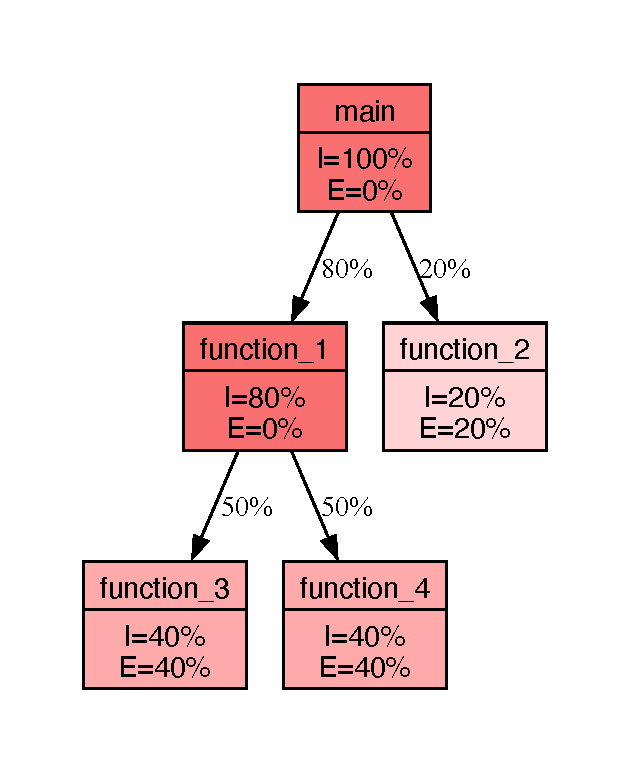
\includegraphics[width=\textwidth, page=1]{Bilder/pdf/profiler_output_example.pdf}
        \caption{Beispielausgabe}\label{fig:beispielausgabe_hana_profiler}
    \end{subfigure}
    \hfill
    \begin{subfigure}[b]{0.45\textwidth}
        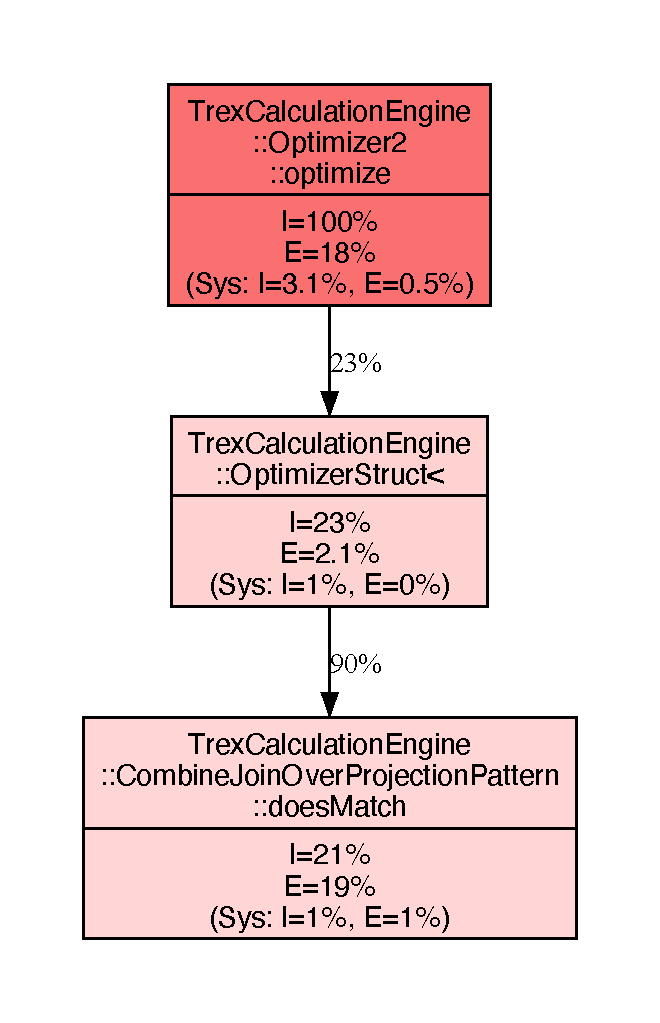
\includegraphics[width=\textwidth, page=1]{Bilder/pdf/2048.1.cpu.pdf}
        \caption{Ausschnitt aus Ausgabe für Messung}\label{fig:profiling_art_1}
    \end{subfigure}
    \caption{Mögliche Ausgaben des HANA-Profilers}\label{fig:profiler_ausgabe}
\end{figure}

% section HANA Profiler (end)
